\documentclass[usenames,dvipsnames,mathserif,notheorems]{beamer}

% silence annoying warnings
\usepackage{silence}
\usepackage{caption}
\WarningFilter{remreset}{The remreset package}
\usepackage{xcolor}

\input{macros/math}
\input{macros/plots}

\usepackage{simplebeam}
\usetheme{simplebeamer}

\usetikzlibrary{shapes, arrows}
\usetikzlibrary{decorations.pathreplacing, calligraphy}

% node styles
\tikzstyle{Input}=[minimum size=0.3cm, fill=black, line width = 0.5mm, draw=black, shape=circle, text=black]
\tikzstyle{Hidden}=[minimum size=0.3cm, fill=blue, line width = 0.5mm, draw=blue, shape=circle, text=black]
\tikzstyle{Splits}=[inner sep=0.03cm, minimum size=0.3cm, line width = 0.3mm, draw=blue, shape=circle, text=black]
\tikzstyle{Output}=[minimum size=0.3cm, fill=white, line width = 0.5mm, draw=black, shape=circle, text=black]

% Edge styles
\tikzstyle{arrow}=[line width = 0.5mm]

% bib resources

\addbibresource[]{refs.bib}

\title{Fast Convex Optimization for Two-Layer ReLU Networks:}
\subtitle{Equivalent Model Classes and Cone Decompositions}
\author{Aaron Mishkin \and Arda Sahiner \and Mert Pilanci}
%\institute{Stanford University}
\collaborators{
		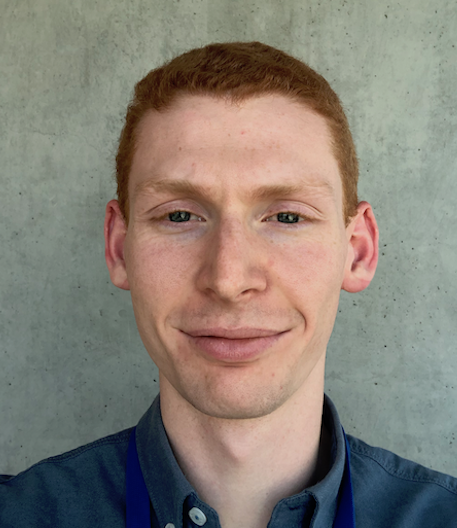
\includegraphics[width=0.2\linewidth]{assets/aaron.png}
		
\includegraphics[width=0.2\linewidth]{assets/arda.jpg}
		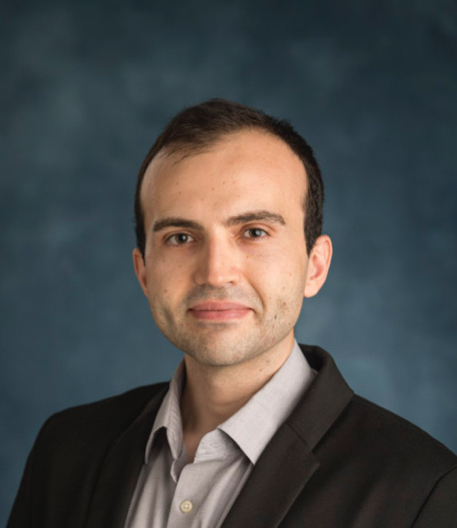
\includegraphics[width=0.2\linewidth]{assets/mert.jpg}
    }

\titlegraphic{
\includegraphics[width=0.4\textwidth]{assets/SUSig_2color_Stree_Left.eps}}

\newcommand{\centerrule}{
	{
	\vspace{-0.5em}
	\center \rule{\textwidth}{0.1em}
	\vspace{-0.2em}
	}
}

%\logo{
\includegraphics[height=0.5cm]{assets/Block_S_2_color.eps}}

%\institute{Stanford University}
\date{}

\begin{document}

\maketitle
%% main content starts %%

\begin{frame}{Overview}

	{
		\large \textcolor{red}{Problem}: Training shallow neural networks is challenging.
	}
	\vspace{0.5em}

	\pause
	\begin{itemize}
		\item \textbf{Tuning}: step-size and other hyper-parameters must be tuned.
		      \pause
		\item \textbf{Model Churn}: models trained with different random seeds
		      have different performance \citep{henderson2018deep}.
		      \pause
		\item \textbf{Certificates}: final models have few guarantees.
	\end{itemize}

	\pause

	\centerrule
	{
		\large \textcolor{ForestGreen}{Our Contribution}: robust training by convex reformulations.
	}
	\vspace{0.5em}
	\pause
	\begin{itemize}
		\item We develop new convex reformulations of two-layer neural networks
		      with \textbf{gated ReLU} activations.
		      \pause
		\item We show how to approximate the ReLU training problem by \textbf{unconstrained}
		      convex optimization of a Gated ReLU network.
		      \pause
		\item We propose and \textbf{exhaustively evaluate} algorithms for solving
		      our convex reformulations.
	\end{itemize}

\end{frame}

\begin{frame}{Background on Convex Reformulations}

	\vspace{0.2em}
	{\large \textcolor{Red}{Non-Convex Problem}}
	\vspace{-1em}
	\begin{columns}
		\centering
		\begin{column}{0.2\linewidth}
			\small
			\[
				\begin{aligned}
					\min_{W} & \norm{\sum_{j=1}^m (X W_{1j})_+ w_{2j} - y}_2^2                  \\
					         & \quad + \lambda \sum_{j=1}^m \norm{W_{1j}}_2^2 + \norm{w_{2j}}^2
				\end{aligned}
			\]
		\end{column}

		\begin{column}{0.7\linewidth}
			\begin{figure}[t]
				\raggedleft
				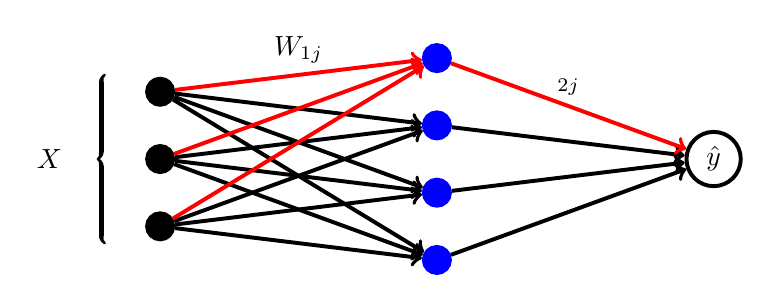
\begin{tikzpicture}[scale=1,
	]
	\begin{axis}[width=\linewidth, height=5cm,
			axis lines=none,  % don't print axis lines
			yticklabels={,,}, xticklabels={,,},
			ymin=0, ymax=8, y axis line style={-},
			xmin=0, xmax=15, x axis line style={-},
		]
		\node [] (input) at (axis cs:1,4) {$X$};
		\node [Input] (input1) at (axis cs:3,2) {};
		\node [Input] (input2) at (axis cs:3,4) {};
		\node [Input] (input3) at (axis cs:3,6) {};

		\draw [decorate, line width = 0.6mm,
			decoration = {calligraphic brace}] (axis cs:2,1.5) --  (axis cs:2,6.5);

		\node [Hidden] (hidden1) at (axis cs:8,1) {};
		\node [Hidden] (hidden2) at (axis cs:8,3) {};
		\node [Hidden] (hidden3) at (axis cs:8,5) {};
		\node [Hidden] (hidden4) at (axis cs:8,7) {};

		\draw [->, style=arrow, draw=black] (input1) -- (hidden1);
		\draw [->, style=arrow, draw=black] (input2) -- (hidden1);
		\draw [->, style=arrow, draw=black] (input3) -- (hidden1);

		\draw [->, style=arrow, draw=black] (input1) -- (hidden2);
		\draw [->, style=arrow, draw=black] (input2) -- (hidden2);
		\draw [->, style=arrow, draw=black] (input3) -- (hidden2);

		\draw [->, style=arrow, draw=black] (input1) -- (hidden3);
		\draw [->, style=arrow, draw=black] (input2) -- (hidden3);
		\draw [->, style=arrow, draw=black] (input3) -- (hidden3);

		\draw [->, style=arrow, draw=red] (input1) -- (hidden4);
		\draw [->, style=arrow, draw=red] (input2) -- (hidden4);
		\draw [->, style=arrow, draw=red] (input3) -- (hidden4) node[pos=0.5,above] {$W_{1j}$};

		\node [Output] (output) at (axis cs:13,4) {$\hat y$};

		\draw [->, style=arrow, draw=black] (hidden1) -- (output);
		\draw [->, style=arrow, draw=black] (hidden2) -- (output);
		\draw [->, style=arrow, draw=black] (hidden3) -- (output);
        \draw [->, style=arrow, draw=red] (hidden4) -- (output) node[pos=0.5,above] {$\w_{2j}$};
	\end{axis}

\end{tikzpicture}%

%\begin{tikzpicture}[scale=1,
%    ]
%    \begin{axis}[width=1.1\linewidth, height=5cm,
%            axis lines=none,  % don't print axis lines
%            yticklabels={,,}, xticklabels={,,},
%            ymin=-0.2, ymax=10.2, x axis line style={-},
%            xmin=-0.2, xmax=20.2, y axis line style={-},
%        ]

%        \filldraw[color=blue!60, fill=blue!5, line width=0.4mm](axis cs:0,5.8) rectangle (axis cs:20, 10);
%        \filldraw[color=red!60, fill=red!5, line width=0.4mm](axis cs:0,0) rectangle (axis cs:20, 4.2);

%        % non-convex models
%        \filldraw[line width=0.4mm, fill=white](axis cs:1,1) rectangle (axis cs:8, 3.2) node[pos=.5] {NC-GReLU};
%        \filldraw[line width=0.4mm, fill=white](axis cs:12,1) rectangle (axis cs:19, 3.2) node[pos=.5] {NC-ReLU};

%        % convex models
%        \filldraw[line width=0.4mm, fill=white](axis cs:1,6.8) rectangle (axis cs:8, 9) node[pos=.5] {C-GReLU};
%        \filldraw[line width=0.4mm, fill=white](axis cs:12,6.8) rectangle (axis cs:19, 9) node[pos=.5] {C-ReLU};

%        \draw [<->, solid, draw=black, line width = 0.6mm] (axis cs:4.5,3.2) -- (axis cs:4.5,6.8) node[right, pos=0.5] {\small Sol. Map};

%        \draw [<->, solid, draw=black, line width = 0.6mm] (axis cs:15.5,3.2) -- (axis cs:15.5,6.8)  node[right, pos=0.5] {\small Sol. Map};

%        \draw [<-, solid, draw=black, line width = 0.6mm] (axis cs:6,9) -- [bend left=15] (axis cs:14, 9);

%        \draw [->, solid, draw=orange, line width = 0.6mm] (axis cs:8,7.9) -- (axis cs:12,7.9);
%        \node[align=center] at (axis cs:10.1, 7.8) {\small Cone\\ \small Decomp.};
%    \end{axis}

%\end{tikzpicture}%


			\end{figure}
		\end{column}
	\end{columns}


	\pause
	\centerrule


	{\large \textcolor{ForestGreen}{Convex Reformulation}} \citep{pilanci2020convex}
	\vspace{-2em}
	\begin{columns}
		\begin{column}{0.2\linewidth}
			\vspace{1.5em}
			\small
			\[
				\begin{aligned}
					\min_{v, w} & \norm{\sum_{j=1}^p D_j X (v_j - w_j) - y}_2^2                       \\
					            & \hspace{0.1em } + \lambda \sum_{j=1}^p \norm{v_j}_2 + \norm{w_j}_2, \\
					            & \hspace{0.1em} \text{s.t. }
					v_j, w_j \in \calK_j \text{ for } j = 1,\ldots,p.
				\end{aligned}
			\]
		\end{column}
		\begin{column}{0.7\linewidth}
			\vspace{-1.5em}
			\begin{figure}[t]
				\raggedleft
				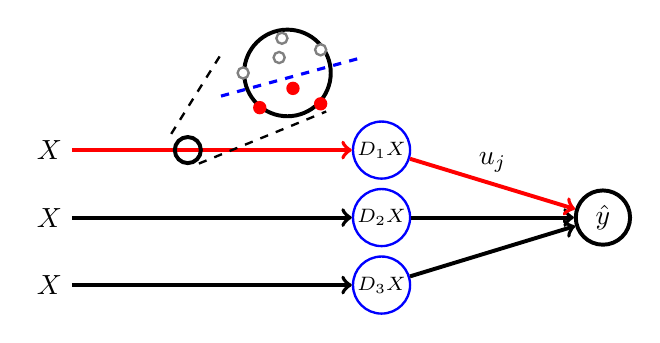
\begin{tikzpicture}[scale=1,
	]
	\begin{axis}[width=\linewidth, height=5.5cm,
			axis lines=none,  % don't print axis lines
			yticklabels={,,}, xticklabels={,,},
			ymin=0, ymax=8, y axis line style={-},
			xmin=0, xmax=15, x axis line style={-},
		]
		\node [] (input1) at (axis cs:3,1) {$X$};
		\node [] (input2) at (axis cs:3,2.75) {$X$};
		\node [] (input3) at (axis cs:3,4.5) {$X$};

        \node [Splits] (hidden1) at (axis cs:9,1) {\scriptsize $D_3 X$};
		\node [Splits] (hidden2) at (axis cs:9,2.75) {\scriptsize $D_2 X$};
		\node [Splits] (hidden3) at (axis cs:9,4.5) {\scriptsize $D_1 X$};

		\draw [->, style=arrow, draw=black] (input1) -- (hidden1);

		\draw [->, style=arrow, draw=black] (input2) -- (hidden2);

		\draw [->, style=arrow, draw=red] (input3) -- (hidden3);

		\node [Output] (output) at (axis cs:13,2.75) {$\hat y$};

		\draw [->, style=arrow, draw=black] (hidden1) -- (output);
		\draw [->, style=arrow, draw=black] (hidden2) -- (output);
		\draw [->, style=arrow, draw=red] (hidden3) -- (output) node[pos=0.5,above] {$u_j$};

		\draw [draw=black, line width=0.3mm, dashed] (axis cs:5.7, 4.15) -- (axis cs:8,5.5);
		\draw [draw=black, line width=0.3mm, dashed] (axis cs:5.2, 4.92) -- (axis cs:6.15,7.1);

		\node [draw=black, minimum size=0.3cm, shape=circle, solid, line width=0.5mm] (examine) at (axis cs:5.5,4.5) {};
		\node [draw=black, minimum size=1.1cm, shape=circle, solid, line width=0.5mm] (closeup) at (axis cs:7.3,6.5) {};

		\node [fill=white, draw=gray, line width=0.3mm, inner sep=0.05cm, shape=circle] at (axis cs:7.9,7.1) {};
		\node [fill=white, draw=gray, line width=0.3mm, inner sep=0.05cm, shape=circle] at (axis cs:7.15,6.9) {};
		\node [fill=white, draw=gray, line width=0.3mm, inner sep=0.05cm, shape=circle] at (axis cs:7.2,7.4) {};
		\node [fill=white, draw=gray, line width=0.3mm, inner sep=0.05cm, shape=circle] at (axis cs:6.5,6.5) {};

		\draw [draw=Blue, dashed, line width=0.4mm] (axis cs:6.1,5.9) -- (axis cs:8.65,6.9);

		\node [fill=Red, inner sep=0.06cm, shape=circle] at (axis cs:6.8,5.6) {};
		\node [fill=Red, inner sep=0.06cm, shape=circle] at (axis cs:7.4,6.1) {};
		\node [fill=Red, inner sep=0.06cm, shape=circle] at (axis cs:7.9,5.7) {};

	\end{axis}

\end{tikzpicture}%

			\end{figure}
		\end{column}
	\end{columns}
\end{frame}

\begin{frame}{Background on Convex Reformulations}

	\vspace{0.2em}
	{\large Non-Convex Problem}
	\vspace{-1em}
	\begin{columns}
		\centering
		\begin{column}{0.2\linewidth}
			\small
			\[
				\begin{aligned}
					\min_{W} & \norm{\sum_{j=1}^m (X W_{1j})_+ w_{2j} - y}_2^2                  \\
					         & \quad + \lambda \sum_{j=1}^m \norm{W_{1j}}_2^2 + \norm{w_{2j}}^2
				\end{aligned}
			\]
		\end{column}

		\begin{column}{0.7\linewidth}
			\begin{figure}[t]
				\raggedleft
				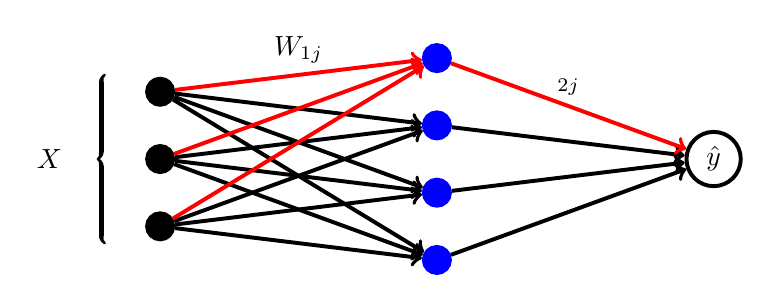
\begin{tikzpicture}[scale=1,
	]
	\begin{axis}[width=\linewidth, height=5cm,
			axis lines=none,  % don't print axis lines
			yticklabels={,,}, xticklabels={,,},
			ymin=0, ymax=8, y axis line style={-},
			xmin=0, xmax=15, x axis line style={-},
		]
		\node [] (input) at (axis cs:1,4) {$X$};
		\node [Input] (input1) at (axis cs:3,2) {};
		\node [Input] (input2) at (axis cs:3,4) {};
		\node [Input] (input3) at (axis cs:3,6) {};

		\draw [decorate, line width = 0.6mm,
			decoration = {calligraphic brace}] (axis cs:2,1.5) --  (axis cs:2,6.5);

		\node [Hidden] (hidden1) at (axis cs:8,1) {};
		\node [Hidden] (hidden2) at (axis cs:8,3) {};
		\node [Hidden] (hidden3) at (axis cs:8,5) {};
		\node [Hidden] (hidden4) at (axis cs:8,7) {};

		\draw [->, style=arrow, draw=black] (input1) -- (hidden1);
		\draw [->, style=arrow, draw=black] (input2) -- (hidden1);
		\draw [->, style=arrow, draw=black] (input3) -- (hidden1);

		\draw [->, style=arrow, draw=black] (input1) -- (hidden2);
		\draw [->, style=arrow, draw=black] (input2) -- (hidden2);
		\draw [->, style=arrow, draw=black] (input3) -- (hidden2);

		\draw [->, style=arrow, draw=black] (input1) -- (hidden3);
		\draw [->, style=arrow, draw=black] (input2) -- (hidden3);
		\draw [->, style=arrow, draw=black] (input3) -- (hidden3);

		\draw [->, style=arrow, draw=red] (input1) -- (hidden4);
		\draw [->, style=arrow, draw=red] (input2) -- (hidden4);
		\draw [->, style=arrow, draw=red] (input3) -- (hidden4) node[pos=0.5,above] {$W_{1j}$};

		\node [Output] (output) at (axis cs:13,4) {$\hat y$};

		\draw [->, style=arrow, draw=black] (hidden1) -- (output);
		\draw [->, style=arrow, draw=black] (hidden2) -- (output);
		\draw [->, style=arrow, draw=black] (hidden3) -- (output);
        \draw [->, style=arrow, draw=red] (hidden4) -- (output) node[pos=0.5,above] {$\w_{2j}$};
	\end{axis}

\end{tikzpicture}%

%\begin{tikzpicture}[scale=1,
%    ]
%    \begin{axis}[width=1.1\linewidth, height=5cm,
%            axis lines=none,  % don't print axis lines
%            yticklabels={,,}, xticklabels={,,},
%            ymin=-0.2, ymax=10.2, x axis line style={-},
%            xmin=-0.2, xmax=20.2, y axis line style={-},
%        ]

%        \filldraw[color=blue!60, fill=blue!5, line width=0.4mm](axis cs:0,5.8) rectangle (axis cs:20, 10);
%        \filldraw[color=red!60, fill=red!5, line width=0.4mm](axis cs:0,0) rectangle (axis cs:20, 4.2);

%        % non-convex models
%        \filldraw[line width=0.4mm, fill=white](axis cs:1,1) rectangle (axis cs:8, 3.2) node[pos=.5] {NC-GReLU};
%        \filldraw[line width=0.4mm, fill=white](axis cs:12,1) rectangle (axis cs:19, 3.2) node[pos=.5] {NC-ReLU};

%        % convex models
%        \filldraw[line width=0.4mm, fill=white](axis cs:1,6.8) rectangle (axis cs:8, 9) node[pos=.5] {C-GReLU};
%        \filldraw[line width=0.4mm, fill=white](axis cs:12,6.8) rectangle (axis cs:19, 9) node[pos=.5] {C-ReLU};

%        \draw [<->, solid, draw=black, line width = 0.6mm] (axis cs:4.5,3.2) -- (axis cs:4.5,6.8) node[right, pos=0.5] {\small Sol. Map};

%        \draw [<->, solid, draw=black, line width = 0.6mm] (axis cs:15.5,3.2) -- (axis cs:15.5,6.8)  node[right, pos=0.5] {\small Sol. Map};

%        \draw [<-, solid, draw=black, line width = 0.6mm] (axis cs:6,9) -- [bend left=15] (axis cs:14, 9);

%        \draw [->, solid, draw=orange, line width = 0.6mm] (axis cs:8,7.9) -- (axis cs:12,7.9);
%        \node[align=center] at (axis cs:10.1, 7.8) {\small Cone\\ \small Decomp.};
%    \end{axis}

%\end{tikzpicture}%


			\end{figure}
		\end{column}
	\end{columns}

	\centerrule

	{\large Convex Reformulation} \citep{pilanci2020convex}
	\vspace{-2em}
	\begin{columns}
		\begin{column}{0.2\linewidth}
			\vspace{1.5em}
			\small
			\[
				\begin{aligned}
					\min_{v, w} & \norm{\sum_{j=1}^p D_j X (v_j - w_j) - y}_2^2                       \\
					            & \hspace{0.1em } + \lambda \sum_{j=1}^p \norm{v_j}_2 + \norm{w_j}_2, \\
					            & \hspace{0.1em}
					\textcolor{red}{\text{s.t. }
						v_j, w_j \in \calK_j \text{ for } j = 1,\ldots,p
					}.
				\end{aligned}
			\]
		\end{column}
		\begin{column}{0.7\linewidth}
			\vspace{-1.5em}
			\begin{figure}[t]
				\raggedleft
				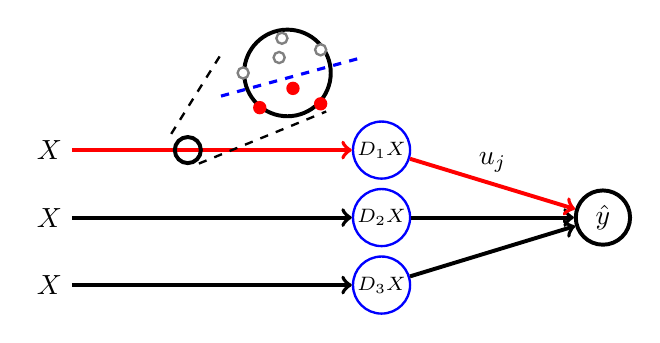
\begin{tikzpicture}[scale=1,
	]
	\begin{axis}[width=\linewidth, height=5.5cm,
			axis lines=none,  % don't print axis lines
			yticklabels={,,}, xticklabels={,,},
			ymin=0, ymax=8, y axis line style={-},
			xmin=0, xmax=15, x axis line style={-},
		]
		\node [] (input1) at (axis cs:3,1) {$X$};
		\node [] (input2) at (axis cs:3,2.75) {$X$};
		\node [] (input3) at (axis cs:3,4.5) {$X$};

        \node [Splits] (hidden1) at (axis cs:9,1) {\scriptsize $D_3 X$};
		\node [Splits] (hidden2) at (axis cs:9,2.75) {\scriptsize $D_2 X$};
		\node [Splits] (hidden3) at (axis cs:9,4.5) {\scriptsize $D_1 X$};

		\draw [->, style=arrow, draw=black] (input1) -- (hidden1);

		\draw [->, style=arrow, draw=black] (input2) -- (hidden2);

		\draw [->, style=arrow, draw=red] (input3) -- (hidden3);

		\node [Output] (output) at (axis cs:13,2.75) {$\hat y$};

		\draw [->, style=arrow, draw=black] (hidden1) -- (output);
		\draw [->, style=arrow, draw=black] (hidden2) -- (output);
		\draw [->, style=arrow, draw=red] (hidden3) -- (output) node[pos=0.5,above] {$u_j$};

		\draw [draw=black, line width=0.3mm, dashed] (axis cs:5.7, 4.15) -- (axis cs:8,5.5);
		\draw [draw=black, line width=0.3mm, dashed] (axis cs:5.2, 4.92) -- (axis cs:6.15,7.1);

		\node [draw=black, minimum size=0.3cm, shape=circle, solid, line width=0.5mm] (examine) at (axis cs:5.5,4.5) {};
		\node [draw=black, minimum size=1.1cm, shape=circle, solid, line width=0.5mm] (closeup) at (axis cs:7.3,6.5) {};

		\node [fill=white, draw=gray, line width=0.3mm, inner sep=0.05cm, shape=circle] at (axis cs:7.9,7.1) {};
		\node [fill=white, draw=gray, line width=0.3mm, inner sep=0.05cm, shape=circle] at (axis cs:7.15,6.9) {};
		\node [fill=white, draw=gray, line width=0.3mm, inner sep=0.05cm, shape=circle] at (axis cs:7.2,7.4) {};
		\node [fill=white, draw=gray, line width=0.3mm, inner sep=0.05cm, shape=circle] at (axis cs:6.5,6.5) {};

		\draw [draw=Blue, dashed, line width=0.4mm] (axis cs:6.1,5.9) -- (axis cs:8.65,6.9);

		\node [fill=Red, inner sep=0.06cm, shape=circle] at (axis cs:6.8,5.6) {};
		\node [fill=Red, inner sep=0.06cm, shape=circle] at (axis cs:7.4,6.1) {};
		\node [fill=Red, inner sep=0.06cm, shape=circle] at (axis cs:7.9,5.7) {};

	\end{axis}

\end{tikzpicture}%

			\end{figure}
		\end{column}
	\end{columns}
\end{frame}

\begin{frame}{Gated ReLU Networks}

	\[
		\begin{aligned}
			\textcolor{Red}{\text{C-ReLU}}: \min_{v, w} & \norm{\sum_{j=1}^p D_j X (v_j - w_j) - y}_2^2
			+ \lambda \sum_{j=1}^p \norm{v_j}_2 + \norm{w_j}_2,                                         \\
			                                            & \hspace{0.1em}
			\textcolor{red}{\text{s.t. }
				v_j, w_j \in \calK_j \text{ for } j = 1,\ldots,p
			}.
		\end{aligned}
	\]
	\pause
	\centerrule
	\[
		\begin{aligned}
			\textcolor{ForestGreen}{\text{C-GReLU}}: \min_{u} & \norm{\sum_{j=1}^p D_j X u_j - y}_2^2
			+ \lambda \sum_{j=1}^p \norm{u_j}_2,                                                      \\
		\end{aligned}
	\]
	\pause
    \vspace{1em}

	\textbf{Prop.} (informal): C-GReLU is equivalent to a ``gated ReLU'' network \citep{fiat2019decoupling}
	with activation function
	\[ \phi_{g}(X, u) = \text{diag}(\mathbbm{1}(Xg \geq 0)) X u. \]

\end{frame}

\begin{frame}{Gated ReLU: Cone Decompositions}
	\begin{itemize}
		\item We reparameterized as \( \textcolor{ForestGreen}{u_j} = \textcolor{Red}{v_j - w_j} \). \pause
		\item Given, \( \textcolor{ForestGreen}{u_j} \), can we go back to \( \textcolor{Red}{v_j - w_j} \)? \pause
		\item That is, when does \( \textcolor{Red}{\calK_j - \calK_j} \) span \( \R^d \)? \pause
	\end{itemize}

	\begin{figure}[]
		\centering
		%! TEX root = ../../main.tex

%% Illustration of cone decomposition. 

\begin{tikzpicture}[scale=1,
		declare function={
				cone_u(\x)= -\x/3;
				cone_l(\x)= -4*\x/5;
			}
	]
    \begin{axis}[width=0.9\linewidth, height=6cm,
			axis lines=center, yticklabels={,,}, xticklabels={,,},
			ymin=-4, ymax=4, ytick={-5,...,5}, ylabel=$$, x axis line style={-},
				xmin=-6, xmax=6, xtick={-5,...,5}, xlabel=$$, y axis line style={-},
		]
		\addplot[name path=cone_u, domain=-6:6, samples=100, line width=1pt]{cone_u(x)};
		\addplot[name path=cone_l, domain=-6:6, samples=200, line width=1pt]{cone_l(x)};

		% add color fill to both cones.
		\addplot fill between[
				of = cone_u and cone_l,
				split, % calculate segments
				every even segment/.style = {fill=blue, fill opacity=0.3},
				every odd segment/.style  = {fill=teal, fill opacity=0.3}
			];

		%% point labels
		% origin point
		\node[circle, fill, inner sep=1pt] at (axis cs:0,0) {};

		\node[label={0:$u_j$}, circle, fill, inner sep=1.8pt] (u) at (axis cs:2,1) {};
		\node[label={90:$v_j$}, circle, fill, inner sep=1.8pt] (v) at (axis cs:25/7+2, -25/21 - 2/3) {};
		\node[label={90:$w_j$}, circle, fill, inner sep=1.8pt] (w) at (axis cs:-25/7, 20/7) {};

		% labels
		\node[label={0:$\calK_j$}] at (axis cs:4,-2.5) {};
		\node[label={180:$-\calK_j$}] at (axis cs:-3.75,2.5) {};
        
        % lines
		\draw [->, dashed, draw=red, line width = 0.4mm] (u) edge (w);
		\draw [->, dashed, draw=red, line width = 0.4mm] (u) edge (v);
	\end{axis}

\end{tikzpicture}%

	\end{figure}
	\pause

	\begin{center}
		\textbf{Informal Result}: \( \textcolor{Red}{\calK_j - \calK_j} = \R^d \) or \( \calK_j \) is ``unimportant''.
	\end{center}
\end{frame}

\begin{frame}{Main Approximation Result}
	\begin{center}
		We can decompose a Gated ReLU neuron into two ReLU neurons.
	\end{center}
	\pause
	\begin{theorem}[Approximation by Cone Decomposition]
		Let \( \lambda \geq 0 \) and let \( p^* \) be the optimal value of the ReLU problem.
		There exists a C-GReLU problem with minimizer \( u^* \) and optimal value \( d^* \) satisfying,
		\[
			d^* \leq p^* \leq d^* + \textcolor{Red}{2 \lambda \kappa(\tilde X_{\calJ}) \sum_{D_i \in \tilde \calD} \norm{u_i^*}_2}.
		\]
	\end{theorem}
	\pause

	{\large Additional Consequences}
	\begin{itemize}
		\item The approximation is exact for \textbf{unregularized} models!
		\item The Gated ReLU and ReLU models are formally \textbf{equivalent}!
	\end{itemize}
\end{frame}

\begin{frame}{Solving the Convex Programs}
	\begin{figure}[]
		\centering
		%! TEX root = ../../main.tex

%% illustration of relations between hypothesis classes. 

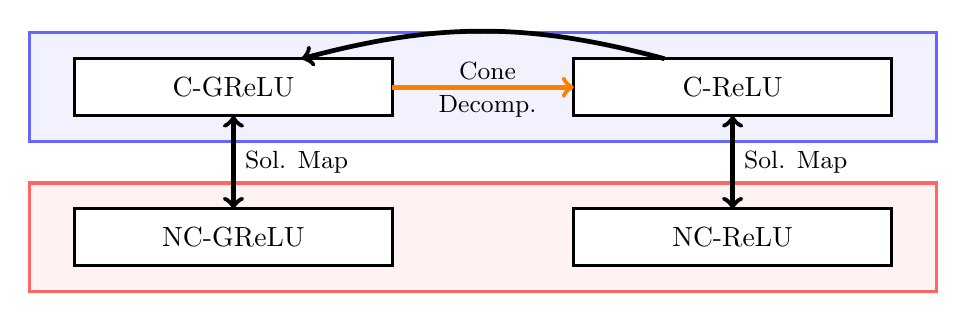
\begin{tikzpicture}[scale=1,
	]
	\begin{axis}[width=1.1\linewidth, height=5cm,
			axis lines=none,  % don't print axis lines
			yticklabels={,,}, xticklabels={,,},
			ymin=-0.2, ymax=10.2, x axis line style={-},
			xmin=-0.2, xmax=20.2, y axis line style={-},
		]

		\filldraw[color=blue!60, fill=blue!5, line width=0.4mm](axis cs:0,5.8) rectangle (axis cs:20, 10);
		\filldraw[color=red!60, fill=red!5, line width=0.4mm](axis cs:0,0) rectangle (axis cs:20, 4.2);

		% non-convex models
		\filldraw[line width=0.4mm, fill=white](axis cs:1,1) rectangle (axis cs:8, 3.2) node[pos=.5] {NC-GReLU};
		\filldraw[line width=0.4mm, fill=white](axis cs:12,1) rectangle (axis cs:19, 3.2) node[pos=.5] {NC-ReLU};

		% convex models
		\filldraw[line width=0.4mm, fill=white](axis cs:1,6.8) rectangle (axis cs:8, 9) node[pos=.5] {C-GReLU};
		\filldraw[line width=0.4mm, fill=white](axis cs:12,6.8) rectangle (axis cs:19, 9) node[pos=.5] {C-ReLU};

		\draw [<->, solid, draw=black, line width = 0.6mm] (axis cs:4.5,3.2) -- (axis cs:4.5,6.8) node[right, pos=0.5] {\small Sol. Map};

		\draw [<->, solid, draw=black, line width = 0.6mm] (axis cs:15.5,3.2) -- (axis cs:15.5,6.8)  node[right, pos=0.5] {\small Sol. Map};

        \draw [<-, solid, draw=black, line width = 0.6mm] (axis cs:6,9) to [bend left=15] (axis cs:14, 9);

		\draw [->, solid, draw=orange, line width = 0.6mm] (axis cs:8,7.9) -- (axis cs:12,7.9);
		\node[align=center] at (axis cs:10.1, 7.8) {\small Cone\\ \small Decomp.};
	\end{axis}

\end{tikzpicture}%

	\end{figure}
	We develop two algorithms for solving the convex reformulations:
	\begin{itemize}
		\item \textbf{R-FISTA}: a restarted FISTA variant for Gated ReLU.
		\item \textbf{AL}: an augmented Lagrangian method for the (constrained) ReLU Problem.
	\end{itemize}
	Our work exhaustively evaluates the performance of R-FISTA and AL.
\end{frame}

\begin{frame}{Numerical Results}
	\begin{figure}[t]
		\centering
		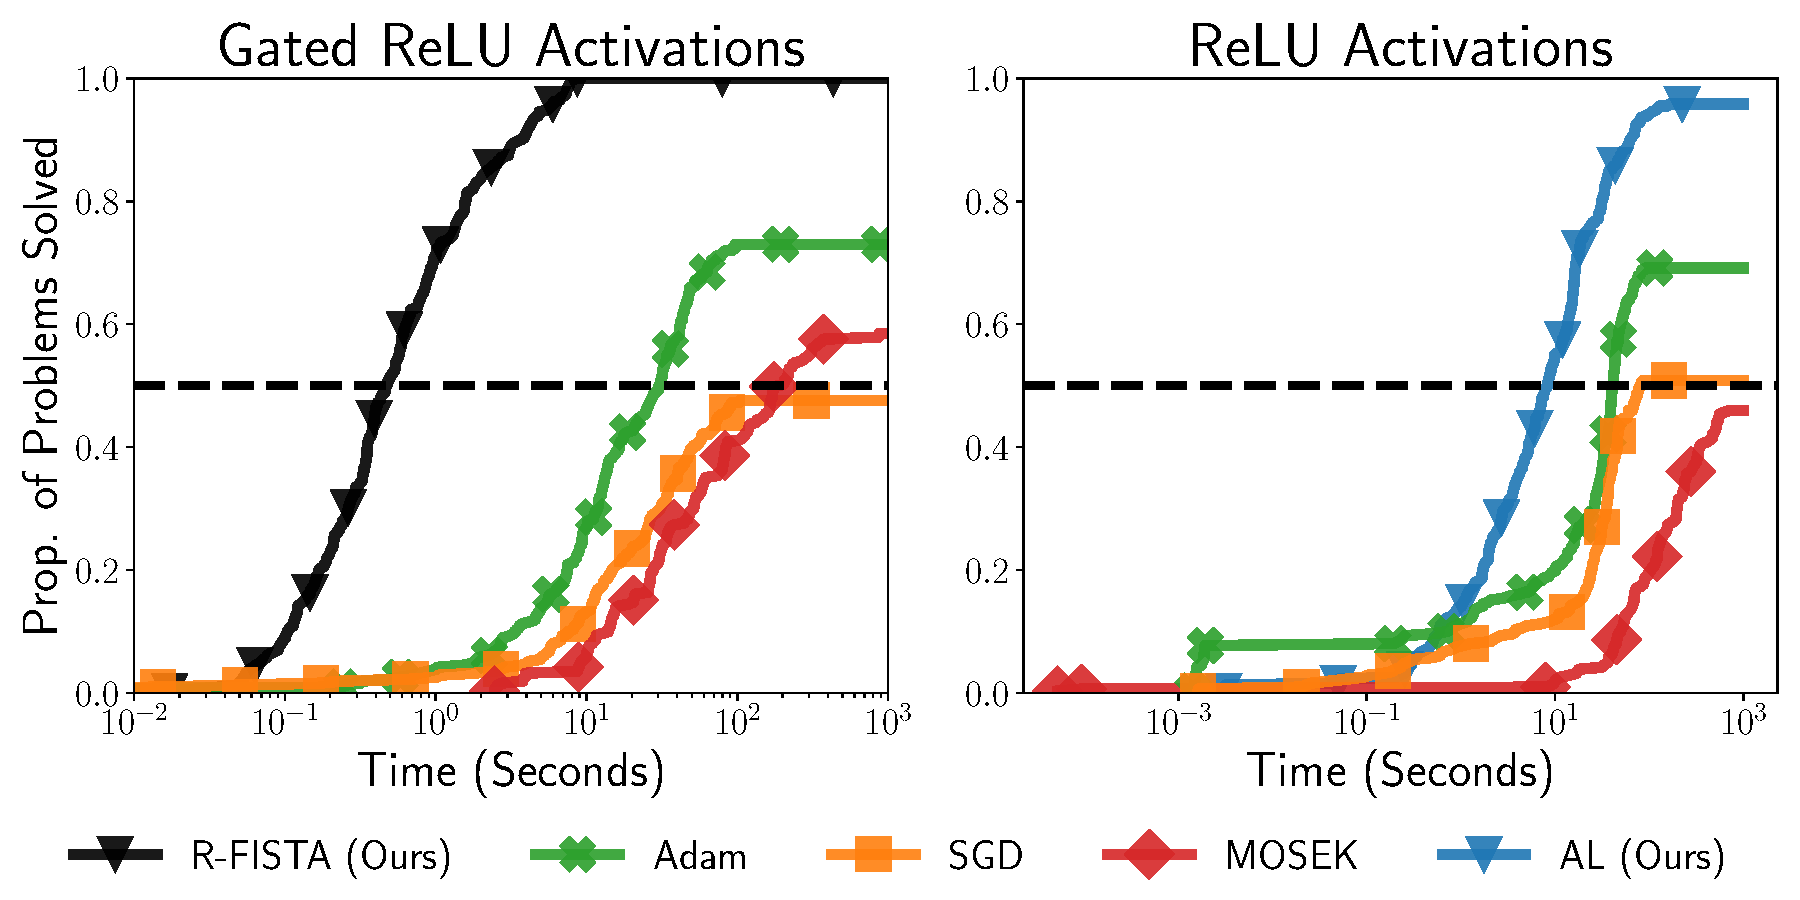
\includegraphics[width=1\linewidth]{assets/pp_main.pdf}
	\end{figure}
	\begin{itemize}
		\item Generated by 438 training problems taken from UCI repo.
		\item R-FISTA/AL solve more, faster, than SGD and Adam.
	\end{itemize}
\end{frame}


%% main content ends %%

%% end slide
\setbeamercolor{background canvas}{bg=LightCyan}

\begin{frame}{}
	\begin{center}
		\huge Thanks for Listening!
	\end{center}
\end{frame}
\setbeamercolor{background canvas}{bg=white}

%% bibliography
\begin{frame}[allowframebreaks]{References}
	\printbibliography[]
\end{frame}


\end{document}
